\clearpage
\myparagraphold{\olly}
\myindex{\olly}

Попробуем этот пример в \olly.
Входное значение функции (2) загружается в \EAX: 

\begin{figure}[H]
\centering
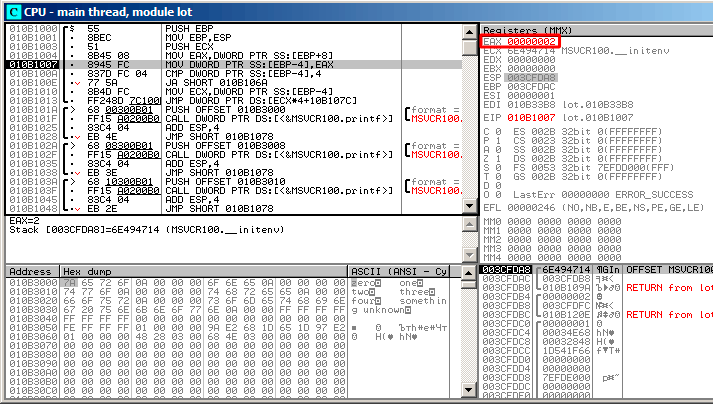
\includegraphics[scale=\FigScale]{patterns/08_switch/2_lot/olly1.png}
\caption{\olly: входное значение функции загружено в \EAX}
\label{fig:switch_lot_olly1}
\end{figure}

\clearpage
Входное значение проверяется, не больше ли оно чем 4? 
Нет, переход по умолчанию (\q{default}) не будет исполнен:

\begin{figure}[H]
\centering
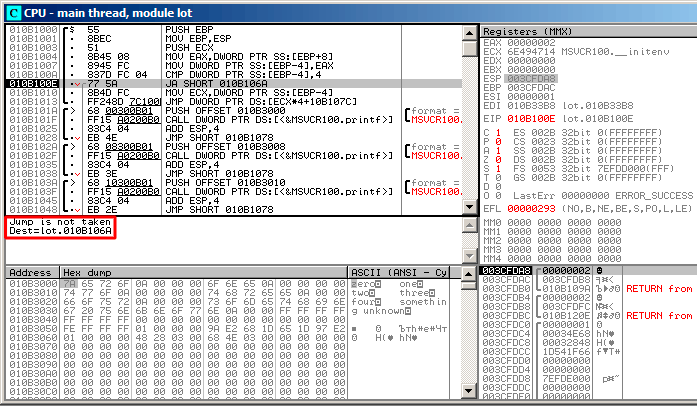
\includegraphics[scale=\FigScale]{patterns/08_switch/2_lot/olly2.png}
\caption{\olly: 2 не больше чем 4: переход не сработает}
\label{fig:switch_lot_olly2}
\end{figure}

\clearpage
Здесь мы видим jumptable:

\begin{figure}[H]
\centering
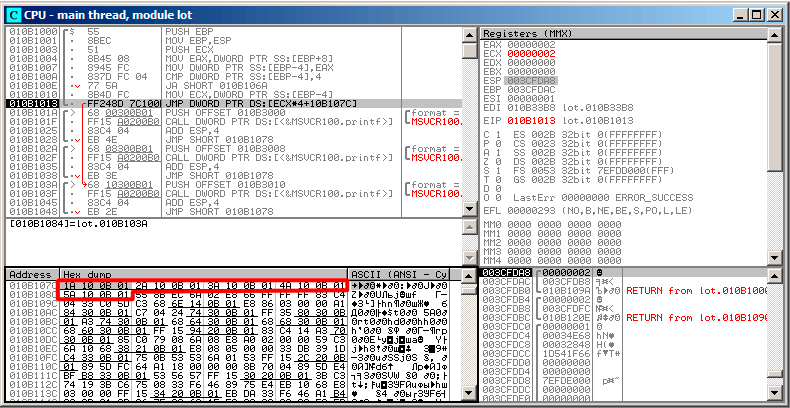
\includegraphics[scale=\FigScale]{patterns/08_switch/2_lot/olly3.png}
\caption{\olly: вычисляем адрес для перехода используя jumptable}
\label{fig:switch_lot_olly3}
\end{figure}

Кстати, щелкнем по \q{Follow in Dump} $\rightarrow$ \q{Address constant}, так что теперь \IT{jumptable} видна в окне данных.

Это 5 32-битных значений\footnote{Они подчеркнуты в \olly, потому что это также и FIXUP-ы: \myref{subsec:relocs}, мы вернемся к ним позже}.
\ECX сейчас содержит 2, так что второй элемент (считая с нулевого) таблицы будет использован.
Кстати, можно также щелкнуть \q{Follow in Dump} $\rightarrow$ \q{Memory address} и \olly покажет элемент, который сейчас адресуется в инструкции \JMP. 
Это \TT{0x010B103A}.

\clearpage
Переход сработал и мы теперь на \TT{0x010B103A}: сейчас будет исполнен код, выводящий строку \q{two}:

\begin{figure}[H]
\centering
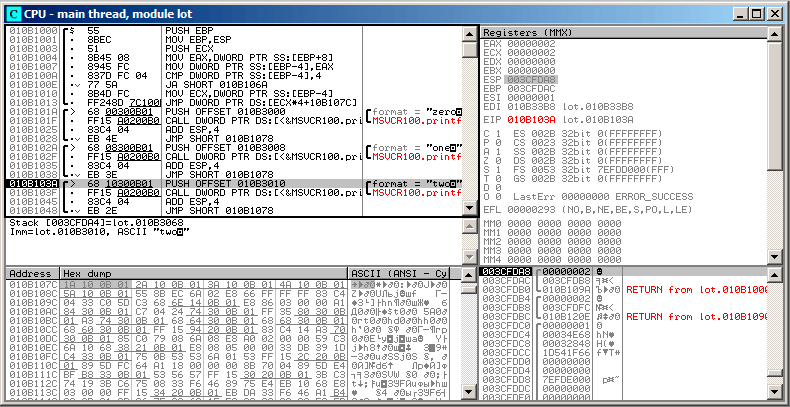
\includegraphics[scale=\FigScale]{patterns/08_switch/2_lot/olly4.png}
\caption{\olly: теперь мы на соответствующей метке \IT{case:}}
\label{fig:switch_lot_olly4}
\end{figure}
